\chapter[Magnituds i comptadors]{Comparació de magnituds i comptadors}
\label{cap:velocitats}

%%--------------------------
%%Posició de totes les llegendes
\pgfplotsset{every axis legend/.append style={
        at={(0.05,0.95)},
        anchor=north west}}
%%--------------------------

Al capítol~\ref{cap:rrdtool-etapes} s'explica profundament com es tracten les dades a RRDtool fins que queden emmagatzemades. Abans de l'etapa de normalització d'intervals, hi ha una etapa de transformació a velocitat que pot quedar descontextualitzada si no s'expliquen els motius històrics que han portat a tractar les dades d'aquesta manera. 

En aquest capítol es raona per què RRDtool té interès a diferenciar variables que classifica com a comptadors i magnituds i per què aplica l'etapa de transformació a velocitat descrita en detall a l'apartat~\ref{sec:rrdtool-etapes:velocitat}. S'anomena velocitat al flux o taxa de variació dels valors quan són expressats com a ràtio magnitud per unitat de temps.


En la primera versió, RRDtool només s'utilitzava per un sistema que monitorava els comptadors de tràfic de xarxa dels encaminadors (\emph{routers}) i els tractava de manera especial, basant-se en la velocitat mitjana del comptador. 
En el primer apartat es resumeix la idea principal d'aquest tractament de velocitat. 

En evolucions posteriors de RRDtool, aquest tractament s'ha mantingut per totes les dades; és a dir que totes les dades es transformen i s'interpreten com a velocitat, fins i tot les que no són comptadors. Es pot concloure que els comptadors han esdevingut el 'cas bàsic' de RRDtool. En un segon apartat s'analitzen les conseqüències que això comporta per a les dades que es mesuren com a magnituds, per exemple la temperatura. 

Al tercer apartat es detallen els noms que utilitza RRDtool per emmagatzemar les variables classificades com a comptadors i com a magnituds i quines possibilitats ofereix per representar-les.

\section{Comptadors}

Com ja s'ha comentat anteriorment, cal situar els inicis de RRDtool en el monitoratge de xarxa de comunicacions amb comptadors. Aquests comptadors són una variable que es va incrementant monòtonament; és a dir són una funció creixent infinita. Per aquesta particularitat, els anomenem comptadors monòtons.

Quan es pren una mesura d'un comptador monòton s'obté un valor que indica el total de comptatge des de l'inici del comptador; és a dir que sempre es mesura amb referència absoluta. 
Per exemple, en diferents instants de temps es prenen mesures d'un comptador de tràfic de xarxa i s'obté el total de bytes que l'encaminador ha processat fins aleshores. A la taula~\ref{tab:velocitats:counter} hi ha unes mesures d'exemple que es poden visualitzar gràficament a la figura~\ref{fig:velocitats:counter}, entre mesures es considera que ha comptat a ritme constant; és a dir linealment.

\begin{table}[tbp]
\centering
\begin{tabular}{c|ccccc}
  temps (s) & 0 & 10 & 20 & 25 & 50 \\ \hline
valor (bytes)& 0 & 1 & 3 & 4 & 10
\end{tabular}
\caption{Mesures d'un comptador monòton}
\label{tab:velocitats:counter}
\end{table}

\begin{figure}[tbp]
  \centering
  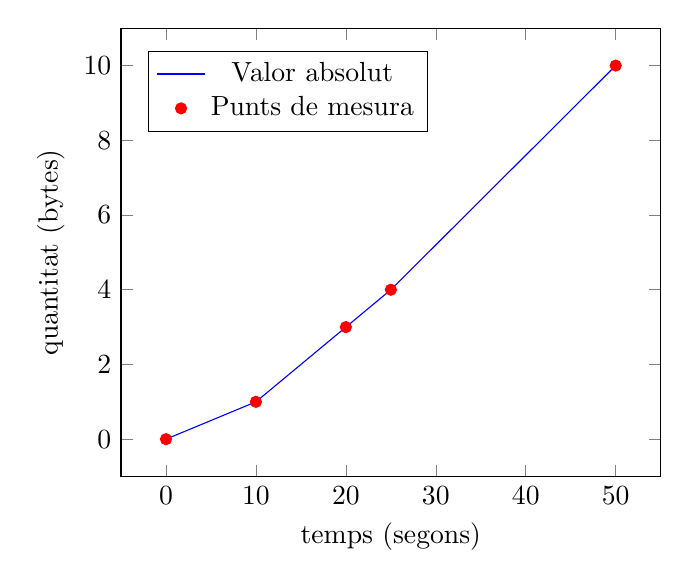
\begin{tikzpicture}
    \begin{axis}[
        xlabel=temps (segons),
        ylabel=quantitat (bytes),
        ]
    \addplot[blue] coordinates {
        (0,0)
        (10,1)
        (20,3)
        (25,4)
        (50,10)
    };
    \addlegendentry{Valor absolut}

    \addplot[only marks,mark=*,red] coordinates {
        (0,0)
        (10,1)
        (20,3)
        (25,4)
        (50,10)
    };
    \addlegendentry{Punts de mesura}

    \end{axis}
  \end{tikzpicture}
  \caption{Evolució del valor d'un comptador monòton}
  \label{fig:velocitats:counter}
\end{figure}



En un pas següent, aquestes mesures preses es poden emmagatzemar a la base de dades, però a RRDtool aquests valors li presenten tres problemes. El primer és que en tractar-se d'una funció sempre creixent, el gràfic que en resulta no és de molta ajuda pels usuaris que l'han d'interpretar. El segon problema és degut a que a la pràctica no es pot comptar fins a un valor infinit sinó que queda acotat en un rang definit per un valor mínim i un valor màxim, anomenat fons d'escala. Així doncs, els comptadors monòtons s'incrementen fins que arriben al fons d'escala i tornen a començar pel valor mínim. Aquest efecte, que s'anomena desbordament, trenca la referència absoluta del comptador, tot i que pot solucionar si el rang del comptador és conegut\footnote{RRDtool només admet valors mínims de 0 i fons d'escala de $2^{32}$ (32 bits) o de $2^{64}$ (64 bits) degut a que fa autodetecció de desbordament per als comptadors d'aparells electrònics, els quals normalment són de 32 o 64 bits.}
i si se suposa que entre dues mesures només hi ha hagut un desbordament (v.\ eq.~\ref{eq:velocitats:increment}). Però aleshores apareix el tercer problema degut a que en les memòries dels computadors tampoc es pot desar un valor infinit.
 
Així doncs, en comptes del valor del comptador es proposa desar els increments del comptador en cada interval, calculats segons l'equació següent:
\begin{equation}\label{eq:velocitats:increment}
\Delta_i = \left\{\begin{array}{ll}
x_i-x_{i-1} & \text{si }  x_{i} \geq x_{i-1} \\
(\text{fons d'escala} -x_{i-1})+ (x_i - \text{valor mínim}) & \text{si }  x_{i} < x_{i-1} 
\end{array}\right.
\end{equation}
on $x_i$ és el valor mesurat en l'instant actual $t_i$, $x_{i-1}$ és el valor mesurat en l'instant anterior $t_{i-1}$ i $\Delta_i$ és l'increment del comptador en l'interval de temps $(t_{i-1},t_i]$.

Aplicant l'equació~\ref{eq:velocitats:increment} a les dades de la taula~\ref{tab:velocitats:counter} s'obtenen els increments per cada interval a la taula~\ref{tab:velocitats:absolute}.

\begin{table}[tbp]
\centering
\begin{tabular}{c|cccc}
  temps (s) & 0-10 & 10-20 & 20-25 & 25-50 \\ \hline
valor (bytes)& 1 & 2 & 1 & 6
\end{tabular}
\caption{Increments d'un comptador monòton}
\label{tab:velocitats:absolute}
\end{table}


\begin{figure}[tbp]
  \centering
  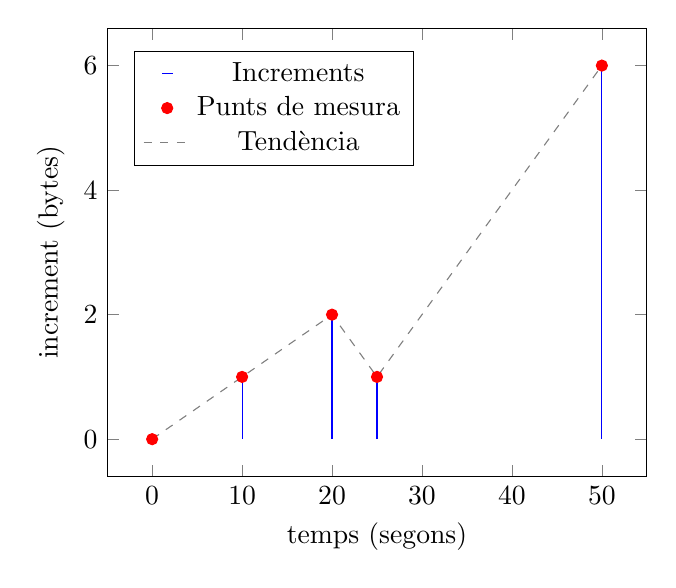
\begin{tikzpicture}
    \begin{axis}[
        xlabel=temps (segons),
        ylabel= increment (bytes)]
    \addplot[ycomb,blue,mark=-] coordinates {
        (0,0)
        (10,1)
        (20,2)
        (25,1)
        (50,6)
    };
    \addlegendentry{Increments}

    \addplot[only marks,mark=*,red] coordinates {
        (0,0)
        (10,1)
        (20,2)
        (25,1)
        (50,6)
    };
    \addlegendentry{Punts de mesura}

    \addplot[gray,dashed] coordinates {
        (0,0)
        (10,1)
        (20,2)
        (25,1)
        (50,6)
    };
    \addlegendentry{Tendència}

    \end{axis}
  \end{tikzpicture}
  \caption{Increments d'un comptador}
  \label{fig:velocitats:deltes}
\end{figure}


A la figura~\ref{fig:velocitats:deltes} es mostra les noves dades calculades en forma d'increments, els quals es representen amb impulsos per reforçar la idea de variable de naturalesa discreta del comptador com a mesurador d'increments. 
També es representa la línia de tendència, tal com es representaria si els increments del comptador provinguessin d'una variable contínua, aquesta línia de tendència dóna una idea de com està evolucionant el comptador. Per un interval concret mostra que si la mesura s'hagués pres a un altre punt, l'increment hauria estat un altre valor, més gran o més petit, però aquesta interpolació queda limitada a l'interval, és a dir que només té sentit una mesura per interval.


Si es vol veure un comptador d'increments com a variable de naturalesa contínua, cal representar-ne el valor relatiu com es fa a la figura~\ref{fig:velocitats:absolute}.
Anomenem valor relatiu al valor del comptador d'increments ja que mostra la quantitat comptada des de l'última mesura. Per representar el valor relatiu, el comptador es posa al valor mínim cada cop que es pren una mesura i se suposa que el comptador s'incrementa linealment, de la mateixa manera que s'ha suposat en el comptador representat en absolut de la figura~\ref{fig:velocitats:counter}.
% Formalment, la primera mesura hauria de ser desconeguda ja que no es coneixen valors anterior al temps 0, i així també passa a RRDtool, però per facilitar la comprensió es considera que el comptador parteix del valor inicial 0.


\begin{figure}[tbp]
  \centering
  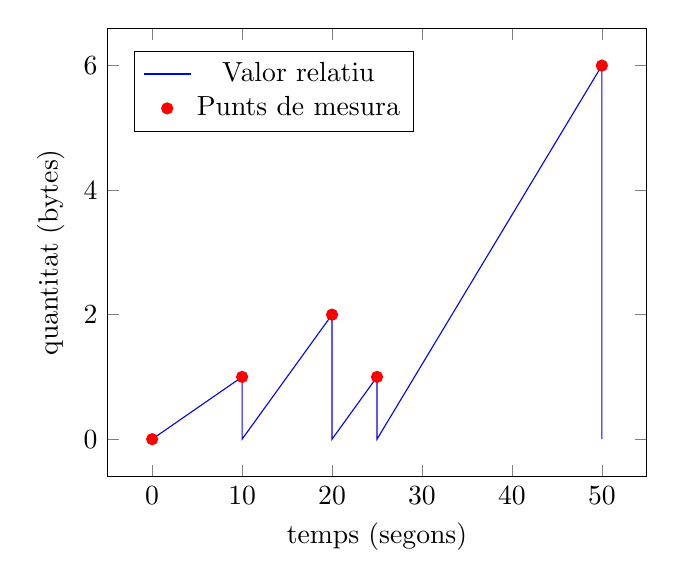
\begin{tikzpicture}
    \begin{axis}[
        xlabel=temps (segons),
        ylabel= quantitat (bytes)]
    \addplot[blue] coordinates {
        (0,0)
        (10,1)
        (10,0)
        (20,2)
        (20,0)
        (25,1)
        (25,0)
        (50,6)
        (50,0)
    };
    \addlegendentry{Valor relatiu}
    \addplot[only marks,mark=*,red] coordinates {
        (0,0)
        (10,1)
        (20,2)
        (25,1)
        (50,6)
    };
    \addlegendentry{Punts de mesura}
    \end{axis}
  \end{tikzpicture}
  \caption{Valor relatiu d'un comptador}
  \label{fig:velocitats:absolute}
\end{figure}

A diferència de la línia de tendència de la figura~\ref{fig:velocitats:deltes}, el valor relatiu sí que pot ser interpolat en més d'un punt de la mateixa manera que el comptador representat en absolut a la  figura~\ref{fig:velocitats:counter}, perquè ambdós només indiquen el valor que es llegirà del comptador en aquell moment.

Per a la interpretació dels increments del comptador, és a dir d'un valor per interval, s'entén més si es representen els valors en un gràfic de barres, com es fa a la figura~\ref{fig:velocitats:barres}. Es representa la freqüència de comptatge per cada interval i també la línia de tendència que s'ha d'interpretar com a la figura~\ref{fig:velocitats:deltes}.

\begin{figure}[tbp]
  \centering
  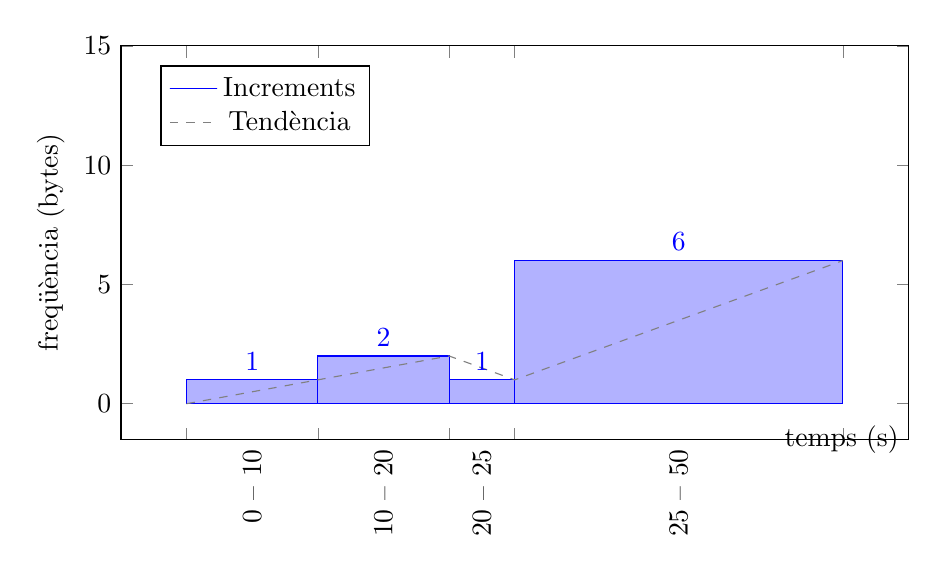
\begin{tikzpicture}
    \begin{axis}[
        width=10cm,scale only axis, height=5cm,
        xlabel=temps (s), 
        ymax = 15,
        ylabel= freqüència (bytes),
        xtick = data,
        xticklabel interval boundaries,
        x tick label style= {rotate=90,anchor=east},
        x label style ={ at={(1,0)},left,yshift=0pt},
        ]
    \addplot[ybar interval,blue,fill=blue!30!white] coordinates{
        (0,1)
        (10,2)
        (20,1)
        (25,6)
        (50,6)
    }; 
    \addlegendentry{Increments}

    \addplot[gray,sharp plot,dashed] coordinates {
        (0,0)
        (10,1)
        (20,2)
        (25,1)
        (50,6)
    };
    \addlegendentry{Tendència}

    \node[color=blue,above] at (axis cs:5,1) {1};
    \node[color=blue,above] at (axis cs:15,2) {2};
    \node[color=blue,above] at (axis cs:22.5,1) {1};
    \node[color=blue,above] at (axis cs:37.5,6) {6};
 
    \end{axis}
  \end{tikzpicture}
  \caption{Gràfic de barres d'increments d'un comptador}
  \label{fig:velocitats:barres}
\end{figure}

En el gràfic de barres a l'eix horitzontal hi ha els intervals representats com a categories de manera que no ajuda a comparar quan hi ha intervals de mida diferent. La proposta següent és dibuixar l'histograma, a on l'àrea de cada barra guarda proporció amb la freqüència de l'interval, com es mostra a la figura~\ref{fig:velocitats:histograma}.

\begin{figure}[tbp]
  \centering
  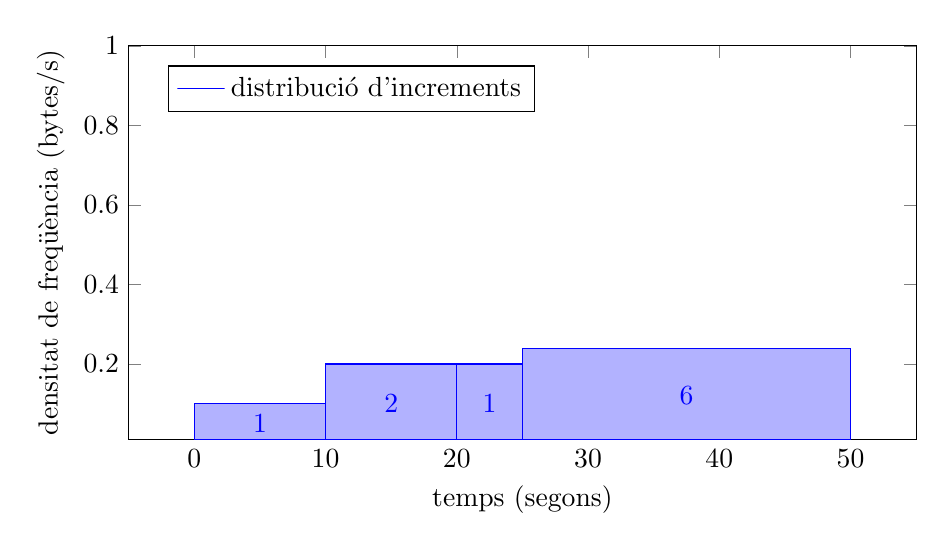
\begin{tikzpicture}
    \begin{axis}[
        width=10cm,scale only axis, height=5cm,
        xlabel=temps (segons),
        ylabel= densitat de freqüència (bytes/s),
        ymax=1,
        ]
    \addplot[ybar interval,blue,fill=blue!30!white,mark=none] coordinates {
        (0,0.1)
        (10,0.2)
        (20,0.2)
        (25,0.24)
        (50,0.24)
    };
    \addlegendentry{distribució d'increments}

    \node[color=blue] at (axis cs:5,0.05) {1};
    \node[color=blue] at (axis cs:15,0.1) {2};
    \node[color=blue] at (axis cs:22.5,0.1) {1};
    \node[color=blue] at (axis cs:37.5,0.12) {6};
 



    \end{axis}
  \end{tikzpicture}
  \caption{Histograma d'increments d'un comptador}
  \label{fig:velocitats:histograma}
\end{figure}

L'histograma en aquest cas és més informatiu pels usuaris ja que es veu el ritme del comptador sense que l'afecti el mostreig  amb mides diferents d'interval.
Els valors de l'eix vertical, la densitat de freqüència de cada interval, estan assenyalant la velocitat mitjana del comptador en cada interval.  De fet, aquesta velocitat mitjana es pot calcular segons l'equació següent:
\begin{equation}\label{eq:velocitats:velocitat}
v_i = 
\frac{\Delta_i}{t_i - t_{i-1}}
\end{equation}
on $\Delta_i$ és l'increment del comptador en l'interval de temps $(t_{i-1},t_i]$  calculat a l'equació~\ref{eq:velocitats:increment}, $t_i$ és l'instant de temps actual, $t_{i-1}$ és l'instant de temps anterior i $v_i$ és la velocitat mitjana del comptador en l'interval de temps $(t_{i-1},t_i]$.

Aplicant l'equació~\ref{eq:velocitats:velocitat} a les dades de la taula~\ref{tab:velocitats:absolute} s'obtenen les velocitats per cada interval a la taula~\ref{tab:velocitats:velocitat}. 
\begin{table}[tbp]
\centering
\begin{tabular}{c|cccc}
  temps (s) & 0-10 & 10-20 & 20-25 & 25-50 \\ \hline
valor (bytes)& 0,1 & 0,2 & 0,2 & 0,24
\end{tabular}
\caption{Velocitats mitjanes d'un comptador monòton}
\label{tab:velocitats:velocitat}
\end{table}

\begin{figure}[tbp]
  \centering
  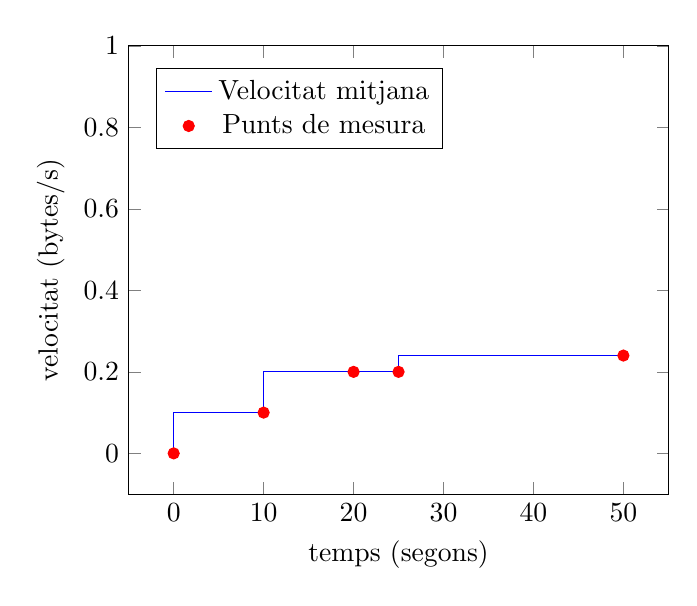
\begin{tikzpicture}
    \begin{axis}[
        xlabel=temps (segons),
        ylabel= velocitat (bytes/s),
        ymax=1,]
    \addplot[const plot mark right,blue] coordinates {
        (0,0)
        (10,0.1)
        (20,0.2)
        (25,0.2)
        (50,0.24)
    };
    \addlegendentry{Velocitat mitjana}

   \addplot[only marks,mark=*,red] coordinates {
        (0,0)
        (10,0.1)
        (20,0.2)
        (25,0.2)
        (50,0.24)
    };
    \addlegendentry{Punts de mesura}

    \end{axis}
  \end{tikzpicture}
  \caption{Velocitat d'un comptador}
  \label{fig:velocitats:velocitat}
\end{figure}

La velocitat mitjana en cada interval s'ha representat a la figura~\ref{fig:velocitats:velocitat} a on s'observa la mateixa forma que a l'histograma de la figura~\ref{fig:velocitats:histograma}, així, tal com passa a l'histograma,  l'àrea del gràfic de velocitat mitjana es correspon a cada interval amb el comptatge incremental i la suma d'increments correspon al comptatge total.
També es pot veure que la velocitat mitjana es correspon amb els pendents aproximats linealment del valor del comptador representat en absolut, figura~\ref{fig:velocitats:counter}, i representat en relatiu, figura~\ref{fig:velocitats:absolute}.


RRDtool decideix emmagatzemar els valors del comptador calculats amb l'equació~\ref{eq:velocitats:velocitat} com a velocitats tot i que podria haver triat l'emmagatzemament dels increments. Segons RRDtool, les velocitats faciliten els càlculs interns que ha de fer la base de dades i es considera que representar la velocitat mitjana és més intuïtiu pels usuaris. 
Per uniformitzar, RRDtool assumeix que les dades emmagatzemades han estat prèviament transformades a velocitat i per tant aplica les operacions i les representacions amb aquesta idea. A continuació es mostra com RRDtool normalitza els interval seguint amb aquesta idea de velocitat i posteriorment es mostra quines conseqüències té per a dades que no són interpretables com a comptador/velocitat, per exemple la temperatura.



\subsection{Normalització}

Una de les parts importants de RRDtool consisteix a normalitzar els intervals per tal que tots tinguin la mateixa durada de temps. L'objectiu és doble: simplificar l'estructura de la base de dades i poder aplicar operacions que necessiten que els intervals siguin regulars.

Com que normalitzar implica canvia els valors del mostreig, s'ha de decidir un criteri per la informació que es vol conservar, per exemple la mitjana o el màxim. RRDtool escull segons el criteri de conservar el comptatge total ja que com s'ha vist abans es desen els comptadors amb la forma de velocitats mitjanes, les àrees de les quals són el comptatge incremental del comptador. 
El criteri del total, també anomenat àrea de sota la corba quan s'aplica a les velocitats mitjanes, és coherent amb els comptadors de tràfic de xarxa ja el primer objectiu d'aquestes base de dades és saber contestar les consultes de quants bytes han circulat entre dos temps.


La normalització a RRDtool es calcula  segons l'explicat a l'apartat~\ref{sec:rrdtool-etapes:normalitzacio}. Per exemple, a la taula~\ref{tab:velocitats:absolute_normal} es normalitzen cada 10 segons els increments de la taula~\ref{tab:velocitats:absolute}. Aquests valors, calculats com a velocitat, són els que s'emmagatzemen a la base de dades.

\begin{table}[tbp]
\centering
\begin{tabular}{c|ccccccc||c}
  temps (s) &  0 & 10 & 20 &25 & 30 & 40 & 50 & total \\ \hline
increments (bytes)& 0 & 1 & 2 & 1 & & & 6 & 10 \\ 
increments normalitzats (bytes)& 0 & 1 & 2 &  & 2,2 & 2,4 & 2,4 & 10
\end{tabular}
\caption{Normalització dels increments d'un comptador monòton}
\label{tab:velocitats:absolute_normal}
\end{table}

Una bona representació gràfica es veu a l'histograma de la figura~\ref{fig:velocitats:histograma_normal}, a on ara  per ser els intervals regulars la forma és molt semblant a un gràfic de barres. 

\begin{figure}[tbp]
  \centering
  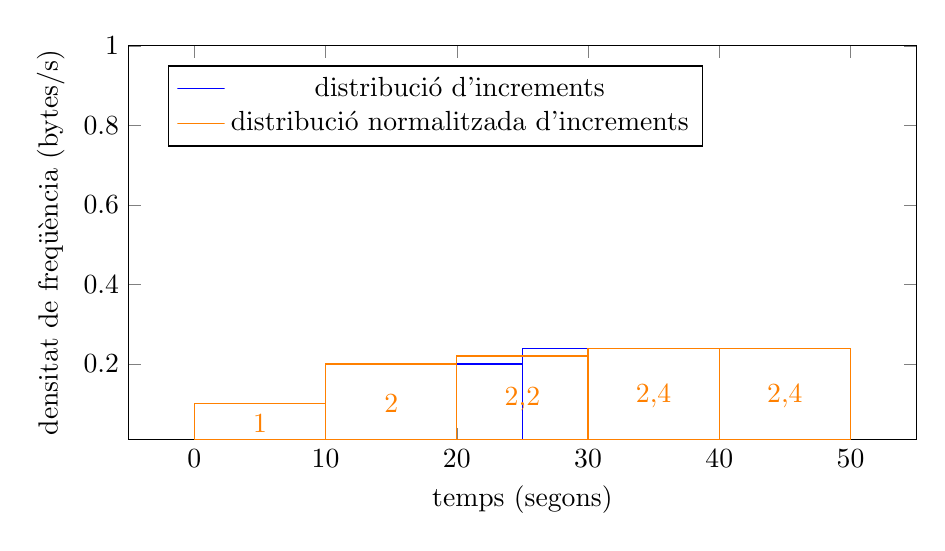
\begin{tikzpicture}
    \begin{axis}[
        width=10cm,scale only axis, height=5cm,
        xlabel=temps (segons),
        ylabel= densitat de freqüència (bytes/s),
        ymax=1,
        ]
    \addplot[ybar interval,blue,mark=none] coordinates {
        (0,0.1)
        (10,0.2)
        (20,0.2)
        (25,0.24)
        (50,0.24)
    };
    \addlegendentry{distribució d'increments}

    \addplot[ybar interval,orange,mark=none] coordinates {
        (0,0.1)
        (10,0.2)
        (20,0.22)
        (30,0.24)
        (40,0.24)
        (50,0.24)
    };
    \addlegendentry{distribució normalitzada d'increments}

    \node[color=orange] at (axis cs:5,0.05) {1};
    \node[color=orange] at (axis cs:15,0.1) {2};
    \node[color=orange] at (axis cs:25,0.11) {2,2};
    \node[color=orange] at (axis cs:35,0.12) {2,4};
    \node[color=orange] at (axis cs:45,0.12) {2,4};
 
    \end{axis}
  \end{tikzpicture}
  \caption{Histograma normalitzat d'increments d'un comptador}
  \label{fig:velocitats:histograma_normal}
\end{figure}

Els valors normalitzats es calculen en valor absolut a la taula~\ref{tab:velocitats:counter_normal} i es representen a la figura~\ref{fig:velocitats:counter_normal}.  El gràfic és el mateix que a la figura~\ref{fig:velocitats:counter} excepte a l'interval de temps $(20,30]$ a on el valor absolut ha canviat de recorregut. Per tant es veu clarament com la normalització de RRDtool reparteix els valors del comptador suposant que s'ha incrementat a velocitat constant i les mostres que queden fora de la linealitat no són recuperables. 


\begin{table}[tbp]
\centering
\begin{tabular}{c|ccccccc}
  temps (s) &  0 & 10 & 20 &25 & 30 & 40 & 50 \\ \hline
valor (bytes)& 0 & 1 & 3 & 4 & & & 10 \\ 
valor normalitzat (bytes)& 0 & 1 & 3 &  & 5,2 & 7,6 & 10
\end{tabular}
\caption{Normalització d'un comptador monòton}
\label{tab:velocitats:counter_normal}
\end{table}

\begin{figure}[tbp]
  \centering
  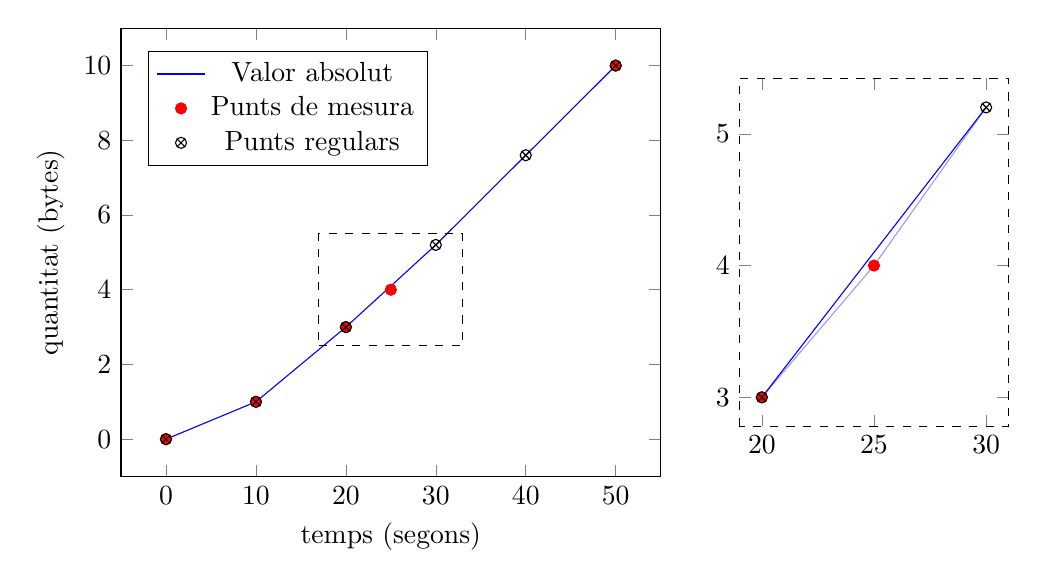
\begin{tikzpicture}
    \usetikzlibrary{calc}
    \begin{axis}[
        name=plot1,
        xlabel=temps (segons),
        ylabel=quantitat (bytes),
        ]
    \addplot[blue] coordinates {
        (0,0)
        (10,1)
        (20,3)
        (30,5.2)
        (50,10)
    };
    \addlegendentry{Valor absolut}

    \addplot[only marks,mark=*,red] coordinates {
        (0,0)
        (10,1)
        (20,3)
        (25,4)
        (50,10)
    };
    \addlegendentry{Punts de mesura}

    \addplot[only marks,mark=otimes,black] coordinates {
        (0,0)
        (10,1)
        (20,3)
        (30,5.2)
        (40,7.6)
        (50,10)
    };
    \addlegendentry{Punts regulars}

    \addplot[black,dashed] coordinates {
        (17,2.5)
        (33,2.5)
        (33,5.5)
        (17,5.5)
        (17,2.5)
    };    

    \end{axis}

\begin{axis}[name=plot2,at={($(plot1.east)+(1cm,0)$)},anchor=west,height=6cm,width=5cm,
    every outer x axis line/.append style=
        {dashed},
    every outer y axis line/.append style=
        {dashed},
]

   \addplot[blue] coordinates {
        (20,3)
        (30,5.2)
    };

   \addplot[blue,opacity=0.4] coordinates {
        (20,3)
        (25,4)
        (30,5.2)
    };
 
   \addplot[only marks,mark=*,red] coordinates {
        (20,3)
        (25,4)
    };
   \addplot[only marks,mark=otimes,black] coordinates {
        (20,3)
        (30,5.2)
    };

\end{axis}


  \end{tikzpicture}
  \caption{Normalització del valor d'un comptador monòton}
  \label{fig:velocitats:counter_normal}
\end{figure}


A la base de dades hi queden emmagatzemats els valors cada 10 segons i el comptatge del comptador ha quedat repartit en aquests intervals segons  el criteri de total per comptadors lineals de RRDtool, descrit a l'apartat~\ref{sec:rrdtool-etapes:normalitzacio}. Ara bé, utilitzant el criteri del total també hi hauria altres normalitzacions possibles, per exemple donant més pes a l'interval amb més comptatge com es fa a l'histograma de la figura~\ref{fig:velocitats:histograma_pes}. El criteri del total el mantinc en els dos casos però un dels dos s'aproxima més al valor que ha tingut el comptador entre els punts de mostreig, els quals són els únics valors que coneixem.

\begin{figure}[tbp]
  \centering
  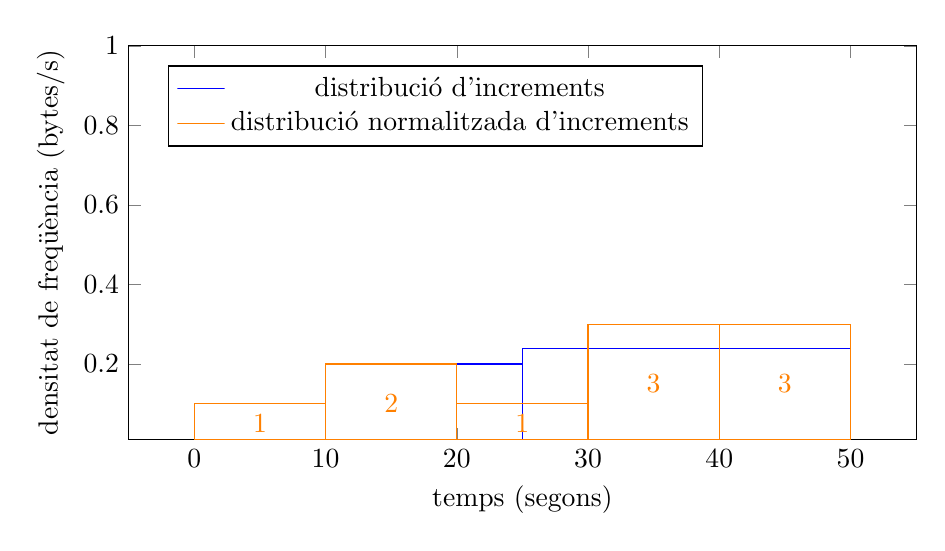
\begin{tikzpicture}
    \begin{axis}[
        width=10cm,scale only axis, height=5cm,
        xlabel=temps (segons),
        ylabel= densitat de freqüència (bytes/s),
        ymax=1,
        ]
    \addplot[ybar interval,blue,mark=none] coordinates {
        (0,0.1)
        (10,0.2)
        (20,0.2)
        (25,0.24)
        (50,0.24)
    };
    \addlegendentry{distribució d'increments}

    \addplot[ybar interval,orange,mark=none] coordinates {
        (0,0.1)
        (10,0.2)
        (20,0.1)
        (30,0.3)
        (40,0.3)
        (50,0.1)
    };
    \addlegendentry{distribució normalitzada d'increments}

    \node[color=orange] at (axis cs:5,0.05) {1};
    \node[color=orange] at (axis cs:15,0.1) {2};
    \node[color=orange] at (axis cs:25,0.05) {1};
    \node[color=orange] at (axis cs:35,0.15) {3};
    \node[color=orange] at (axis cs:45,0.15) {3};
 
    \end{axis}
  \end{tikzpicture}
  \caption{Histograma normalitzat d'increments d'un comptador, donant més pes als darrers intervals}
  \label{fig:velocitats:histograma_pes}
\end{figure}




\subsubsection{Normalització per mitjana}

A l'inici de l'apartat, s'ha dit que RRDtool escull el criteri de total per conservar la informació, però que hi ha altres criteris possibles com la mitjana o el màxim. 
A continuació s'exemplifica una normalització pel criteri de mitjana aritmètica comparada amb una pel criteri de total que fa RRDtool. S'utilitzen les dades del comptador anterior i ara es normalitza amb un sol valor tot l'interval de temps $(0,50]$. Els resultats es poden veure a la taula~\ref{tab:velocitats:counter_criteris} expressats en el domini d'increments i en el domini de velocitats.

\begin{table}[tbp]
\centering
\begin{tabular}{c||c|c}
normalització $(0,50]$  & criteri total  & criteri mitjana  \\ \hline
 & & \\
domini increments (bytes) & $10$  &$\frac{1+2+1+6}{4} = 2{,}5$ \\ 
 & & \\
domini velocitats (bytes/s) & $0{,}2$ & $\frac{ \frac{1}{10} + \frac{2}{10} + \frac{1}{5} +\frac{6}{25} }{4} = 0{,}16$ 
\end{tabular}
\caption{Normalització d'un comptador monòton segons dos criteris}
\label{tab:velocitats:counter_criteris}
\end{table}


La normalització pel criteri total es mostra a l'histograma de la figura~\ref{fig:velocitats:histograma_criteris}. A la figura~\ref{fig:velocitats:counter_criteris} es mostren conjuntament la normalització pel criteri total i pel criteri mitjana representats en valor absolut.
Com que no s'ha de repartir entre dos intervals més petits, en aquest cas el criteri del total es podria haver calculat com la suma d'increments en comptes de la ponderació que fa RRDtool. 


\begin{figure}[tbp]
  \centering
  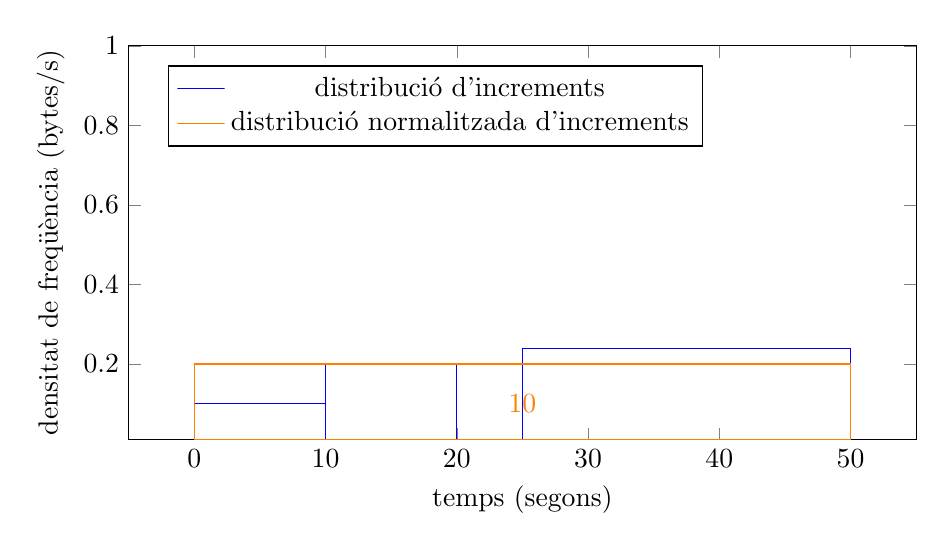
\begin{tikzpicture}
    \begin{axis}[
        width=10cm,scale only axis, height=5cm,
        xlabel=temps (segons),
        ylabel= densitat de freqüència (bytes/s),
        ymax=1,
        ]
    \addplot[ybar interval,blue,mark=none] coordinates {
        (0,0.1)
        (10,0.2)
        (20,0.2)
        (25,0.24)
        (50,0.24)
    };
    \addlegendentry{distribució d'increments}

    \addplot[ybar interval,orange,mark=none] coordinates {
        (0,0.2)
        (50,0.2)
    };
    \addlegendentry{distribució normalitzada d'increments}

    \node[color=orange] at (axis cs:25,0.1) {10};
 
    \end{axis}
  \end{tikzpicture}
  \caption{Histograma normalitzat per tot l'interval d'un comptador}
  \label{fig:velocitats:histograma_criteris}
\end{figure}



\begin{figure}[tbp]
  \centering
  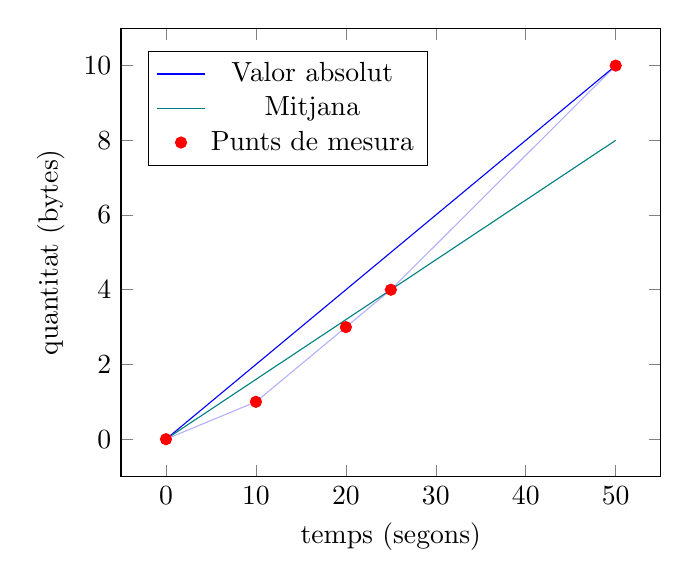
\begin{tikzpicture}
    \begin{axis}[
        xlabel=temps (segons),
        ylabel=quantitat (bytes),
        ]


    \addplot[blue] coordinates {
        (0,0)
        (50,10)
    };
    \addlegendentry{Valor absolut}

    \addplot[teal] coordinates {
        (0,0)
        (50,8)
    };
    \addlegendentry{Mitjana}

    \addplot[only marks,mark=*,red] coordinates {
        (0,0)
        (10,1)
        (20,3)
        (25,4)
        (50,10)
    };
    \addlegendentry{Punts de mesura}

    \addplot[blue,opacity=0.3] coordinates {
        (0,0)
        (10,1)
        (20,3)
        (25,4)
        (50,10)
    };

    \end{axis}
  \end{tikzpicture}
  \caption{Normalització per tot l'interval del valor d'un comptador monòton}
  \label{fig:velocitats:counter_criteris}
\end{figure}


Ens aquests valors es veu com la velocitat mitjana no és el mateix que la mitjana de les velocitats. La velocitat mitjana és el mateix que la mitjana ponderada de les velocitats que és el que fa RRDtool en calcular l'àrea de sota la corba, al qual es pot anomenar criteri del total.
La mitjana aritmètica de les velocitats dóna idea del flux mitjana que hi ha, és a dir que reparteix equitativament la velocitat en el temps. A partir de la mitjana de la velocitat no es pot recuperar el comptatge total, en canvi l'àrea de la velocitat mitjana es correspon exactament amb el total.



\section{Magnituds}

De l'apartat anterior es conclou que el cas bàsic a RRDtool és la velocitat i que es normalitza i representa d'acord amb aquest concepte. Aquest esquema funciona adequadament per variables de naturalesa comptadora, però que passa quan la variable mesurada és una magnitud física, per exemple la temperatura, i per tant no es pot definir com una funció monòtona.

A continuació s'explica com RRDtool emmagatzema magnituds aplicant el seu mètode de normalització pel criteri del total, primer es considera que una magnitud és com un comptador en valor absolut i després es considera que una magnitud és la velocitat d'un comptador.
Es pren com a exemple les mesures de temperatura de la taula~\ref{tab:velocitats:temperatura}. Aquestes mesura es representen a la figura~\ref{fig:velocitats:temperatura}, a on el valor absolut es dibuixa amb interpolacions suavitzades que és la forma que solen tenir les magnituds físiques. 

\begin{table}[tbp]
\centering
\begin{tabular}{c|ccccc}
  temps (s) &  0 & 10 & 20 &25  & 50 \\ \hline
temperatura ($^\circ$C)& 15 & 25 & 15 & 20 & 25 
\end{tabular}
\caption{Valors de temperatura}
\label{tab:velocitats:temperatura}
\end{table}

\begin{figure}[tbp]
  \centering
  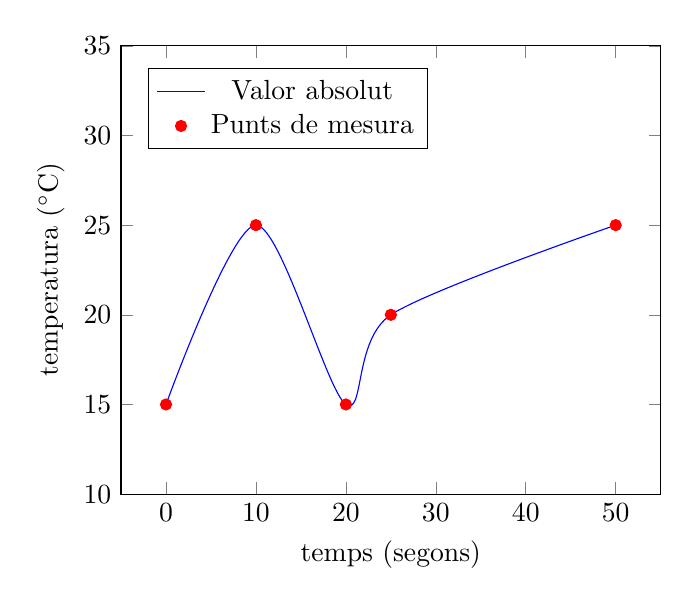
\begin{tikzpicture}
    \begin{axis}[
        ymax = 35,
        ymin = 10,
        xlabel=temps (segons),
        ylabel=temperatura ($^\circ$C),
        ]
    \addplot[blue,smooth] coordinates {
        (0,15)
        (10,25)
        (20,15)
        (25,20)
        (50,25)
    };
    \addlegendentry{Valor absolut}

    \addplot[only marks,mark=*,red] coordinates {
        (0,15)
        (10,25)
        (20,15)
        (25,20)
        (50,25)
    };
    \addlegendentry{Punts de mesura}

    \end{axis}
  \end{tikzpicture}
  \caption{Evolució del valor de temperatura}
  \label{fig:velocitats:temperatura}
\end{figure}

\subsection{Emmagatzematge relatiu}

Seguint amb l'esquema de normalització pels comptadors monòtons, es pot veure el valor absolut de temperatura com un comptador que ara ja no és una funció monòtona sinó que pot ser creixent o decreixent arbitràriament en qualsevol punt. 
Per no ser una funció monòtona ja no hi segueixen havent els mateixos problemes i es podria desar en valor absolut en compres de guardar la velocitat mitjana. Tot i així, RRDtool segueix aplicant els mateixos esquemes encara que en cas de tractar-se de comptadors no monòtons desactiva el detector de desbordaments de l'equació~\ref{eq:velocitats:increment} i permet que tinguin increments negatius, calculats segons l'equació següent:
\begin{equation}\label{eq:velocitats:derive}
\Delta_i = 
x_i-x_{i-1} 
\end{equation}

Aplicant l'equació~\ref{eq:velocitats:derive} a les dades de la taula~\ref{tab:velocitats:temperatura} s'obtenen els increments de temperatura per cada interval a la taula~\ref{tab:velocitats:temperatura_relativa}. 

\begin{table}[tbp]
\centering
\begin{tabular}{c|cccc}
  temps (s) &  0-10 & 10-20 &20-25  & 25-50 \\ \hline
increments ($^\circ$C)& 10 & -10 & 5 & 5 
\end{tabular}
\caption{Increments de temperatura}
\label{tab:velocitats:temperatura_relativa}
\end{table}



\begin{figure}[tbp]
  \centering
  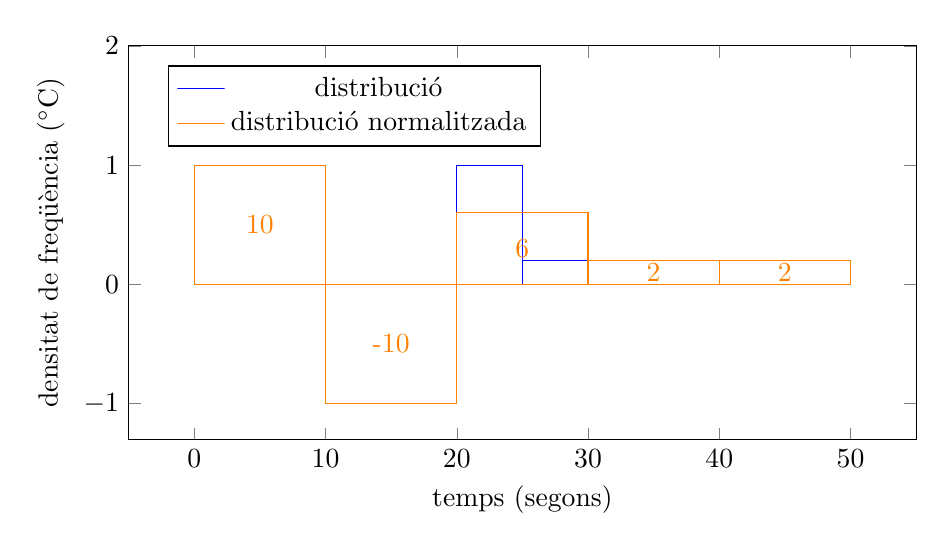
\begin{tikzpicture}
    \begin{axis}[
        width=10cm,scale only axis, height=5cm,
        xlabel=temps (segons),
        ylabel= densitat de freqüència ($^\circ$C),
        ymax=2,
        ]
    \addplot[ybar interval,blue,mark=none] coordinates {
        (0,1)
        (10,-1)
        (20,1)
        (25,0.2)
        (50,0.2)
    };
    \addlegendentry{distribució}

    \addplot[ybar interval,orange,mark=none] coordinates {
        (0,1)
        (10,-1)
        (20,0.6)
        (30,0.2)
        (40,0.2)
        (50,0.2)
    };
    \addlegendentry{distribució normalitzada}

    \node[color=orange] at (axis cs:5,0.5) {10};
    \node[color=orange] at (axis cs:15,-0.5) {-10};
    \node[color=orange] at (axis cs:25,0.3) {6};
    \node[color=orange] at (axis cs:35,0.1) {2};
    \node[color=orange] at (axis cs:45,0.1) {2};
 
    \end{axis}
  \end{tikzpicture}
  \caption{Histograma normalitzat per a increments de temperatura}
  \label{fig:velocitats:histograma_temperatura_relativa}
\end{figure}


A la figura~\ref{fig:velocitats:histograma_temperatura_relativa} es representa la normalització dels increments de temperatura segons el criteri de total vist anteriorment.
En el cas de comptadors no té gaire efecte que siguin monòtons o no ja que d'ambdues maneres es guarda el total i la representació d'increments segueix sent útil. Però en el cas de les magnituds el total perd sentit ja que normalment es vol visualitzar els valors 'tal qual'. En canvi si es desen els increments, es perd la referència i no es poden recuperar els valors originals. És més, els increments de les variables com la temperatura, en total són zero ja que es manté osci\l.lant al voltant d'uns valors de referència. Per extensió, la velocitat mitjana al límit també s'aproxima a zero i aquests són els valors que RRDtool emmagatzema. A la figura~\ref{fig:velocitats:temperatura_increments} es representa el gràfic que RRDtool mostra si es desa la temperatura com a comptador.


\begin{figure}[tbp]
  \centering
  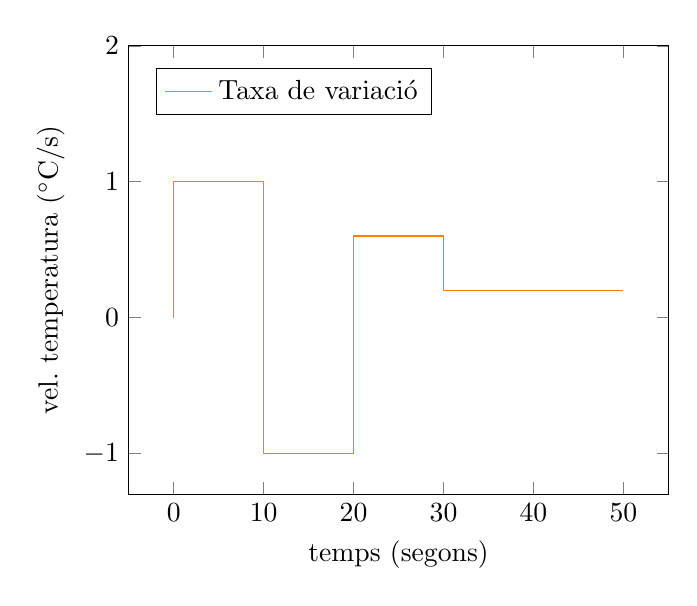
\begin{tikzpicture}
    \begin{axis}[
        ymax = 2,
        xlabel=temps (segons),
        ylabel= vel.\ temperatura ($^\circ$C/s),
        ]


    \addplot[const plot mark right,orange] coordinates {
        (0,0)
        (10,1)
        (20,-1)
        (30,0.6)
        (40,0.2)
        (50,0.2)
    };
    \addlegendentry{Taxa de variació}

    \end{axis}
  \end{tikzpicture}
  \caption{Normalització d'increments de temperatura}
  \label{fig:velocitats:temperatura_increments}
\end{figure}


\subsection{Emmagatzematge absolut}

Així doncs, RRDtool no és capaç de recuperar la referència absoluta si s'emmagatzemen les magnituds com un comptador. La solució que es proposa per part de RRDtool és emmagatzemar les magnituds directament en el domini de velocitats dels comptadors. Aleshores els valors s'emmagatzemen 'tal qual' i s'aplica la normalització seguint l'esquema de RRDtool, de tal manera que els valors de temperatura ara es representen a l'eix de freqüència de l'histograma. Es pot veure un exemple a l'histograma de la figura~\ref{fig:velocitats:histograma_temperatura} a on es normalitzen els valors de temperatura de la taula~\ref{tab:velocitats:temperatura}.


\begin{figure}[tbp]
  \centering
  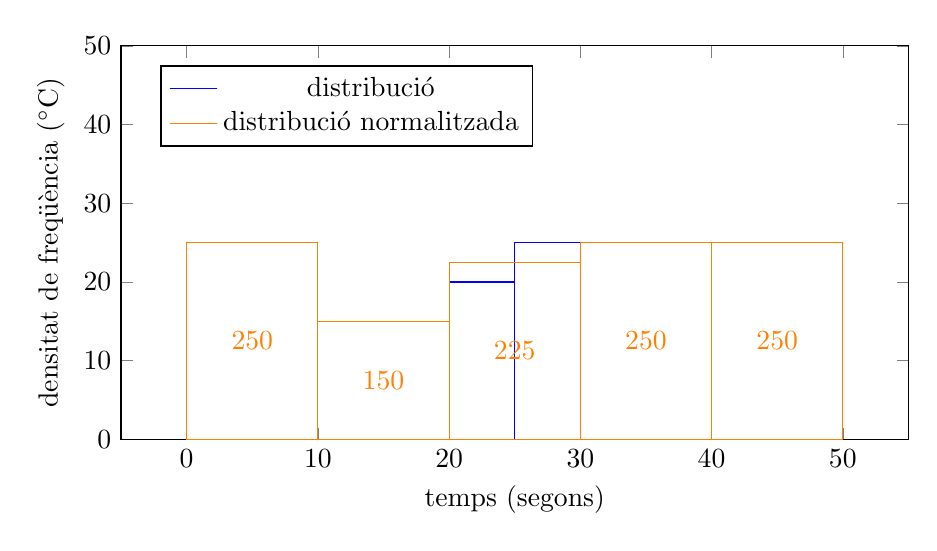
\begin{tikzpicture}
    \begin{axis}[
        width=10cm,scale only axis, height=5cm,
        xlabel=temps (segons),
        ylabel= densitat de freqüència ($^\circ$C),
        ymax=50,
        ymin = 0,
        ]
    \addplot[ybar interval,blue,mark=none] coordinates {
        (0,25)
        (10,15)
        (20,20)
        (25,25)
        (50,25)
    };
    \addlegendentry{distribució}

    \addplot[ybar interval,orange,mark=none] coordinates {
        (0,25)
        (10,15)
        (20,22.5)
        (30,25)
        (40,25)
        (50,25)
    };
    \addlegendentry{distribució normalitzada}

    \node[color=orange] at (axis cs:5,12.5) {250};
    \node[color=orange] at (axis cs:15,7.5) {150};
    \node[color=orange] at (axis cs:25,11.25) {225};
    \node[color=orange] at (axis cs:35,12.5) {250};
    \node[color=orange] at (axis cs:45,12.5) {250};
 
    \end{axis}
  \end{tikzpicture}
  \caption{Histograma normalitzat per a temperatura}
  \label{fig:velocitats:histograma_temperatura}
\end{figure}




\begin{figure}[tbp]
  \centering
  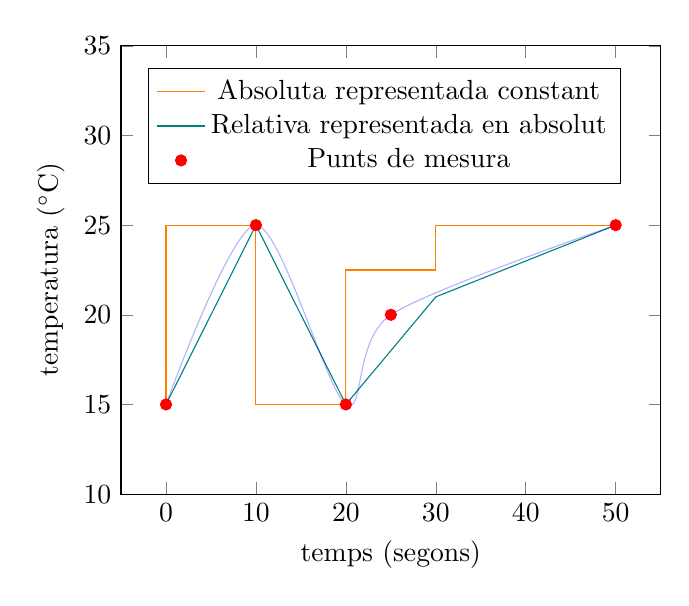
\begin{tikzpicture}
    \begin{axis}[
        ymax = 35,
        ymin = 10,
        xlabel=temps (segons),
        ylabel=temperatura ($^\circ$C),
        ]


    \addplot[const plot mark right,orange] coordinates {
        (0,15)
        (10,25)
        (20,15)
        (30,22.5)
        (40,25)
        (50,25)
    };        
    \addlegendentry{Absoluta representada constant}

    \addplot[teal] coordinates {
        (0,15)
        (10,25)
        (20,15)
        (30,21)
        (40,23)
        (50,25)
    };        
    \addlegendentry{Relativa representada en absolut}


    \addplot[only marks,mark=*,red] coordinates {
        (0,15)
        (10,25)
        (20,15)
        (25,20)
        (50,25)
    };
    \addlegendentry{Punts de mesura}

    \addplot[blue,smooth,opacity=0.3] coordinates {
        (0,15)
        (10,25)
        (20,15)
        (25,20)
        (50,25)
    };



    \end{axis}
  \end{tikzpicture}
  \caption{Comparació normalitzacions del valor de temperatura}
  \label{fig:velocitats:temperatura_criteris}
\end{figure}


A la figura~\ref{fig:velocitats:temperatura_criteris} es compara la temperatura emmagatzemada en relatiu com a comptador i en absolut com a velocitat de comptador. 
La primera variable, en ser un comptador, a RRDtool s'ha emmagatzemat com a velocitat i es representaria com s'ha fet anteriorment a la figura~\ref{fig:velocitats:temperatura_increments}, però en el gràfic actual es representa correctament amb la referència per poder-la comparar en el mateix domini que els valors de temperatura.
La segona variable, per RRDtool  és tractada com una velocitat mitjana i es dibuixa tal com RRDtool la representaria.

L'emmagatzematge de les magnituds tant de la manera relativa com l'absoluta dóna bons resultats d'aproximació. Ara bé, a RRDtool només es poden emmagatzemar com a absoluts ja que no conserva la referència en les relatives.

\section[RRDtool]{Emmagatzematge a RRDtool}

Com s'ha vist al llarg d'aquest capítol, RRDtool va començar sent una base de dades per a comptadors de tràfic de xarxa i per aquesta raó històrica encara avui dia està molt lligat a l'emmagatzematge de dades que tenen naturalesa de comptadors. A més a més, la representació de les dades també està molt lligada als comptadors. Per tant, representació i emmagatzematge estan massa acoblats per a poder comprendre i expandir RRDtool de manera flexible.

L'emmagatzematge dels comptadors es duu a terme en el domini de velocitat, és a dir que donats unes mesures d'un comptador es transformen a velocitat. Depenent de la manera com aquestes mesures es transformen a velocitat, RRDtool classifica els comptadors en quatre tipus:

\begin{itemize}

\item \emph{Counter} és un comptador monòton que es mesura en valor absolut i es transforma segons les equacions~\ref{eq:velocitats:increment} i~\ref{eq:velocitats:velocitat},  com el vist a la figura~\ref{fig:velocitats:counter}.

\item \emph{Absolute} és un comptador, monòton o no, que es mesura en valor relatiu i es transforma segons l'equació~\ref{eq:velocitats:velocitat} , com el monòton vist a la figura~\ref{fig:velocitats:absolute}  i el no monòton vist a la figura~\ref{fig:velocitats:histograma_temperatura_relativa}.

\item \emph{Derive} és un comptador no monòton que es mesura en valor absolut i es transforma segons les equacions~\ref{eq:velocitats:derive} i~\ref{eq:velocitats:velocitat}, com el vist a la figura~\ref{fig:velocitats:temperatura}.

\item \emph{Gauge} és un comptador, monòton o no, del que es mesura la velocitat mitjana en el darrer interval, com el vist a la figura~\ref{fig:velocitats:histograma_temperatura}. Els valors que es mesuren ja són velocitat i per tant no hi ha transformació.

\end{itemize}

L'equació~\ref{eq:velocitats:velocitat} és l'encarregada de transformar els valors mesurats a velocitat mitjana. Com es pot veure, s'aplica als tres primers tipus i per tant es pot dir que qualsevol comptador acaba emmagatzemat amb el valor de la seva velocitat mitjana tal com passa directament en el darrer cas, els \emph{gauge}. En resum, els \emph{gauge} són el cas bàsic a RRDtool a causa de les raons històriques comentades al llarg d'aquest capítol. 

A més a més, la representació que pot fer RRDtool dels comptadors està limitada en aquests valors emmagatzemats; és a dir que només pot mostrar gràfics de l'evolució de la velocitat mitjana, com s'ha vist a les figures ~\ref{fig:velocitats:velocitat} i~\ref{fig:velocitats:temperatura_increments} i en general com s'ha vist als histogrames a on la velocitat mitjana es correspon amb l'eix de densitat de freqüències. 
RRDtool no és capaç de fer representacions dels comptadors en valor absolut a partir de la velocitat mitjana que té emmagatzemada. Tot i així, per una millor comprensió del capítol, 
a les figures \ref{fig:velocitats:counter_normal}, \ref{fig:velocitats:counter_criteris} i~\ref{fig:velocitats:temperatura_criteris} s'han representat els comptadors en valor absolut per poder comparar els valors originals del comptador amb els que s'emmagatzemen, ja que no és possible comparar en un mateix gràfic el domini comptador i el domini velocitat. 


Finalment, s'ha explicat que RRDtool recomana desar les magnituds físiques com a tipus \emph{gauge}. RRDtool només admet els quatre tipus de dades llistats en aquest apartat i els  \emph{gauge} són els que més s'avenen a les magnituds ja que emmagatzemen els valors 'tal qual'. En aquest capítol s'ha explicat com es podria desar una magnitud de manera relativa, com si fos un comptador, però que es perdia la referència absoluta i no es podia recuperar correctament. Aquesta pèrdua de referència també es pot produir en els comptadors,  però en anomenar-los comptadors s'està suposant que el què interessa són justament els valors relatius; és a dir representar els increments als quals RRDtool es troba més còmode representar en velocitat mitjana.






%%% Local Variables: 
%%% mode: latex
%%% TeX-master: "memoria"
%%% End: 

% LocalWords:  RRDtool
